\documentclass{article}

\usepackage{amsmath, amsthm, amssymb}
\usepackage{graphicx, url}

\title{Comprehension 2 for PMCC \\ \small ``Commodity cluster-based parallel
  processing of hyperspectral imagery'' by Antonio Plaza et al.}
\author{Michael Talbot \small $<$tlbmic004$>$ \and Keegan Smith \small
  $<$smtkee002$>$ \and Min-Young Wu \small $<$wxxmin003$>$}

\begin{document}

\maketitle

\section*{Question 1}

\paragraph{(a)}
Due to the increasingly large images that are being captured from satellites,
more and more data needs to be analysed. There are also several applications
where having the results computed in near real-time will be advantageous,
e.g. detecting and/or tracking natural disasters. High performance computing
systems have become increasingly widespread, and these systems offer a means
of analysing the images quickly, provided that a parallel solution is
used. Hence why parallel solutions for hyperspectral imagery is becoming
increasingly needed.

\paragraph{(b)}
See figure \ref{fig:1b}. The arrows indicate the data flow, while the numbers
indicates the flow of control and processing.

\emph{Data flow}: The results from step 2 is divided up (forking arrows) and
sent to the slave threads for processing. The results from the slaves in step
4 are joined together (joining arrows) in step 5 to calculate the covariance
matrix.

\emph{Processing flow}: Step 1 executes, followed by step 2, then step 3.

\paragraph{(c)}
The bottlenecks of the algorithm are:
\begin{itemize}
\item \emph{Step 1}, sending out the K partitions: communication bottleneck.
\item \emph{Step 2}, combining the K unique sets to form the final unique set
  of p unique vectors: synchronisation requirement.
\item \emph{Step 5}, calculating the covariance matrix: synchronisation
  requirement.
\item \emph{Step 6}, obtaining the transformation matrix: serial part.
\item \emph{Step 7}, receiving the transformation matrix: communication
  bottleneck.
\item \emph{Step 8}, combining the results: synchronisation requirement.
\end{itemize}

\begin{figure}[tp]
\centering
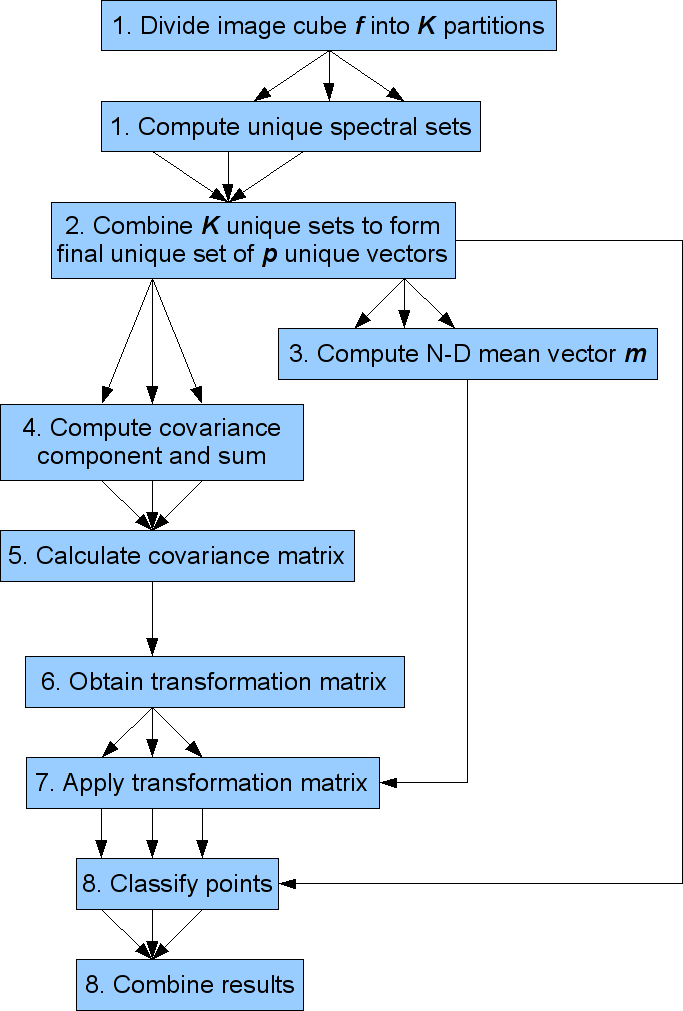
\includegraphics[scale=0.7]{question1_b.png}
\caption{Flow chart for question 1b)}\label{fig:1b}
\end{figure}


\section*{Question 2}

\paragraph{(a)}
See figure \ref{fig:2a}.

\paragraph{(b)}
The initial division of work is a serial part of the algorithm, done by the
master. In step 3, the master has to collect data from all the workers. This
will cause a bottleneck to do with syncronization. Step 4 is a serial
bottleneck because the master has to do the comparison. Step 5 could provide a
bottleneck in communication, but it seems unlikely for a small number of
processors and would only be a problem for large numbers of processors. Step 6
is serial again with the master having to decide on action for each
cluster. Step 7 will probably have a communication bottleneck.

\paragraph{(c)}
Minimising inter-process communication will reduce the number and severity of
bottlenecks. This makes the parallel part of the code proportionally larger,
increasing its scalability.

\begin{figure}[tp]
\centering 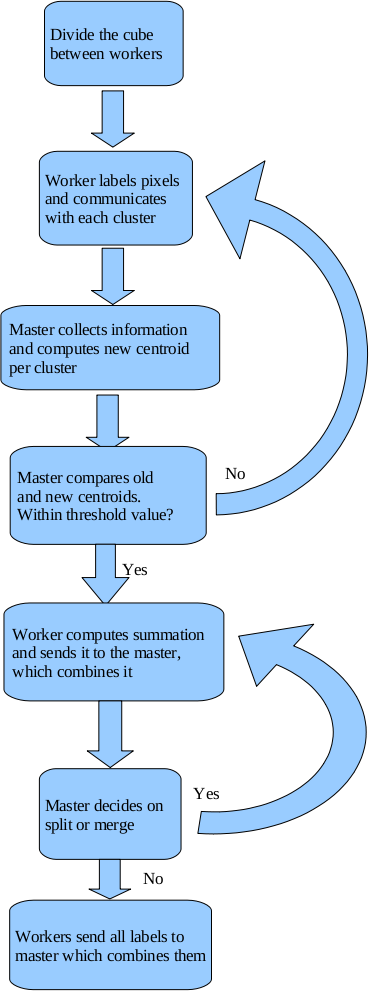
\includegraphics[scale=0.7]{question2_a.png}
\caption{Flow chart for question 2a)}\label{fig:2a}
\end{figure}


\section*{Question 3}

\paragraph{(a)}
See figure \ref{fig:3a}.

\paragraph{(b)}
\begin{itemize}
\item Step 1 is a communication bottleneck since the master has to send
  exactly what each machine needs, instead of using ghost cells.
\item Step 2 processes each PSSP serially, so nodes may finish their work load
  at different times leading to unused processor cycles.
\item There are no synchronisation requirements excluding the obvious waiting
  for all processes to finish at step 3 to reduce results.
\end{itemize}

\paragraph{(c)}
The only group communications are done from master to slaves. This is done
once at the beginning and once at the end. This is advantageous because it
reduces communication and synchronisation bottlenecks during computation. It
also reduces complexity of the code since each slave does no communication
during the computation.

\paragraph{(d)}
Store a non-mutable array of $K$ PSSPs. Then do an OpenMP parallel for loop
from $i=1$ to $K$, where each $i$ runs the serial AMEE algorithm on PSSP
$i$. Store the result in position $i$ in a $K$ sized mutable array. This works
since there is no dependence between each $i$.

\begin{figure}[tp]
\centering 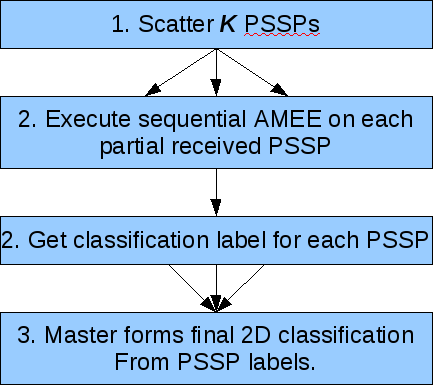
\includegraphics[scale=0.7]{question3_a.png}
\caption{Flow chart for question 3a)}\label{fig:3a}
\end{figure}


\section*{Question 4}

\paragraph{(a)}
Mesh-based parallel architectures is a way of labelling the physical layout of
nodes in a cluster. In this case nodes are laid out in a 2D array, where each
node is linked to the neighbouring 4 nodes.

This is useful architecture for algorithms which use a spatial divisioning of
the data. If the algorithm at a point depends on the other local points, there
is less communication overhead to retrieve the local points. This architecture
would not work where global information, or non-local information is needed
often during the computation.

\paragraph{(b)}
Spatial domain parallelism is better suited to distributed memory
architectures since the work can be divided up such that each node can only
communication to a few local nodes. The most accessed data will be stored in
each nodes memory, exploiting data locality more effectively.

Spectral-domain parallelism requires more global communication between
processes so shared memory machines are better since there is low cost
occurred for any type of communication.

\paragraph{(c)}
AMEEPAR's only communication is at the very beginning and at the very end. So
as expected it scales very well, but not perfectly linearly due to the larger
communication required from the master for more nodes.

S-PCT and D-ISODATA have a good speedup, but not as favourable as
AMEEPAR. This is because more communication and synchronisation happens mid
computation.

\paragraph{(d)}
Including the master in the load-balance analysis for S-PCT and D-ISODATA
significantly degrades the load-balance numbers. This indicates that the
master node is doing too much work. This is due to the sequential steps
necessary in both algorithms. AMEEPAR on the other hand has nearly perfect
load-balance. This is another indication at how well it scales.



\end{document}
